\documentclass[size=14pt,
style=paintings
%style=aggie
%style=bframe
%style=ciment
%style=elcolors
%style=fyma blue
%style=fyma brown
%style=fyma gray
%style=fyma green
%style=fyma orange
%style=horatio
%style=husky
%style=ikeda
%style=jefka blue
%style=jefka brown
%style=jefka seagreen
%style=jefka white
%style=klope blackwhite
%style=klope bluewater
%style=klope pastelflower
%style=klope spring
%style=paintings charon
%style=paintings europa
%style=paintings goldengate
%style=paintings holywood
%style=paintings lamentation
%style=paintings maythird
%style=paintings moitessier
%style=paintings pearlearring
%style=paintings skater
%style=paintings syndics
%style=pazik brown
%style=pazik red
%style=sailor chocolate
%style=sailor cocktail
%style=sailor river
%style=sailor sea
%style=sailor wine
%style=simple
]{powerdot}

\pdsetup{palette=Skater}

\usepackage[utf8]{inputenc}
\usepackage{xcolor}
\title{Introdução ao \LaTeX}

\date{Janeiro, 2014}

\newenvironment{vslide}{\vspace{\stretch{1}}}{\vspace{\stretch{1}}}

\begin{document}
\maketitle

%%-------------------------------------------------------------------------------------
\begin{slide}{\Large A escrita científica}
  \vspace{.2cm}
  % \twocolumn{
  \onslide{2-}{Trabalhos para disciplinas}
  \vspace{1cm}
  
  \onslide{3-}{Relatórios de iniciação científica}
  \vspace{1cm}
  
  \onslide{4-}{Artigos científicos}
  \vspace{1cm}
  
  \onslide{5-}{TCC}
  \vspace{1cm}

  \onslide{6-}{Apresentações}
 \end{slide}

\begin{slide}{\Large As normas, regras, diretrizes}
  \vspace{.2cm}
  % \twocolumn{
  \onslide{2-}{Congressos}
  \vspace{1.5cm}
  
  \onslide{3-}{Professores}
  \vspace{1.5cm}
  
  \onslide{4-}{Banca avaliadora}
  \vspace{1.5cm}
  
  \onslide{5-}{ABNT/SBC/IEEE/ACM}
\end{slide}

 \begin{slide}{\Large Os detalhes}
   \vspace{.2cm}

   \twocolumn[lcolwidth=.30\linewidth,rcolwidth=.70\linewidth]{
   \onslide{2-}{Tipografia}
  \vspace{1.5cm}
  
  \onslide{3-}{Facilidade de leitura}
  \vspace{1.5cm}
  
  \onslide{5-}{Ser entendido}
  \vspace{1.5cm}
  
  \onslide{6-}{Ser ouvido}
}
{
        \begin{figure}[!h]
          \onslide*{2}{ 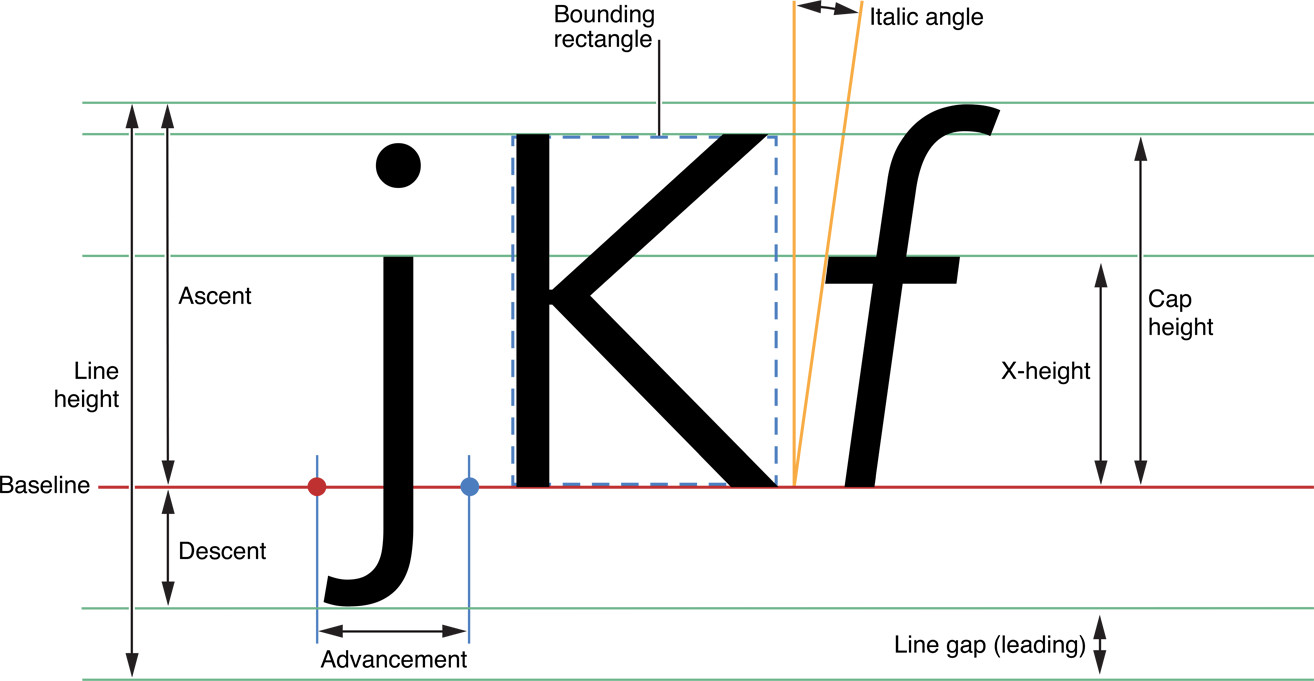
\includegraphics[scale=.14]{resources/typo}}
          \onslide*{3}{ 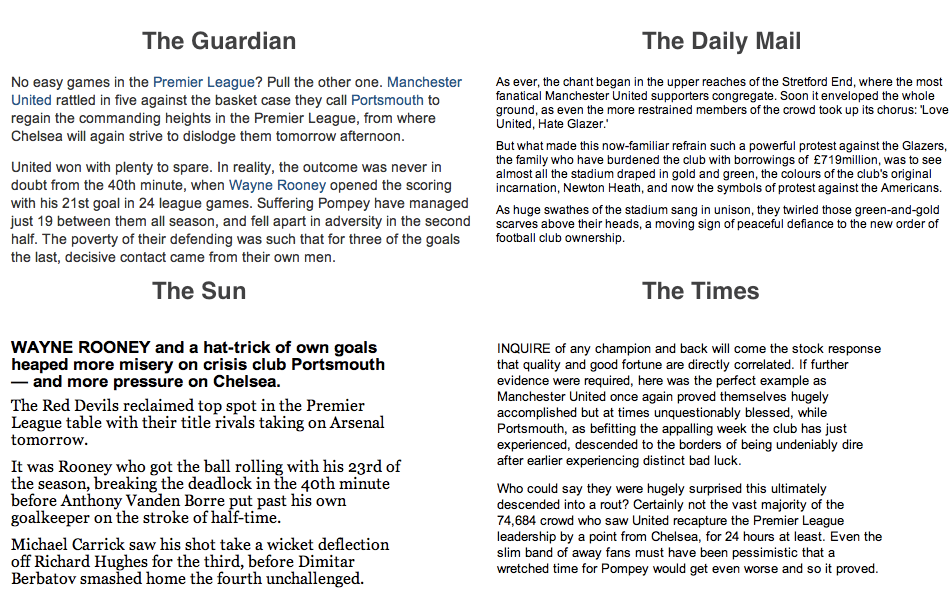
\includegraphics[scale=.28]{resources/comparison}}
          \onslide*{4-}{ 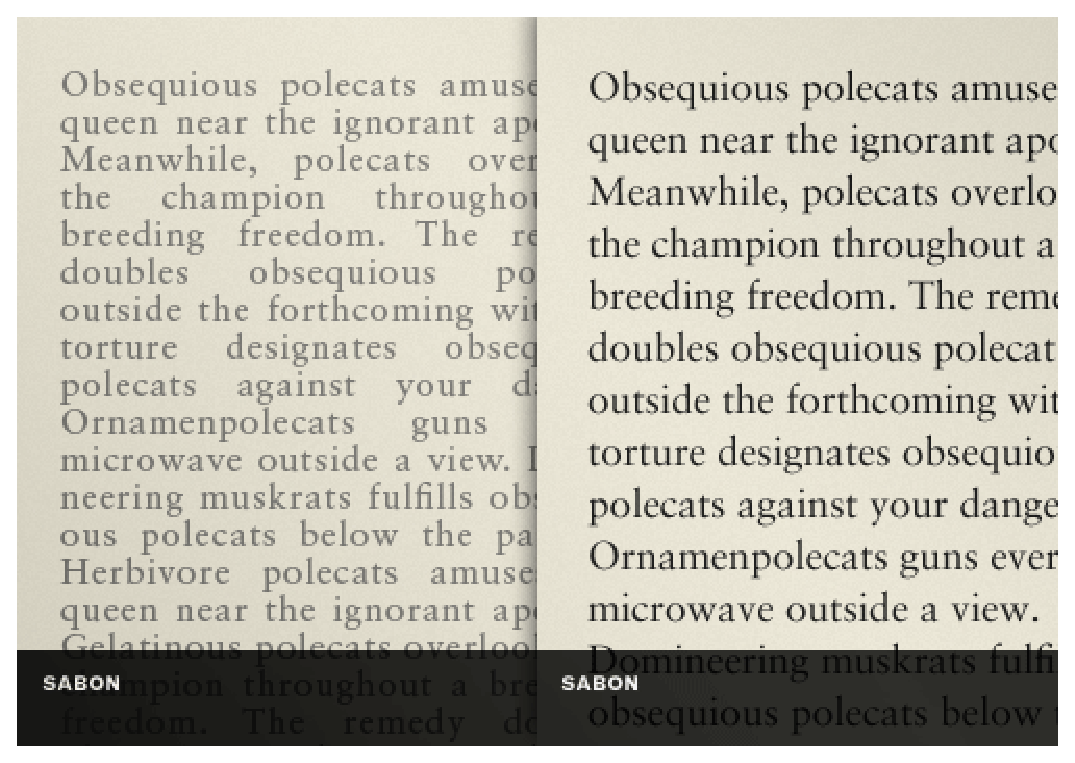
\includegraphics[scale=.4]{resources/readibility}}
        \end{figure}        

        \begin{figure}[!h]
          \onslide*{2}{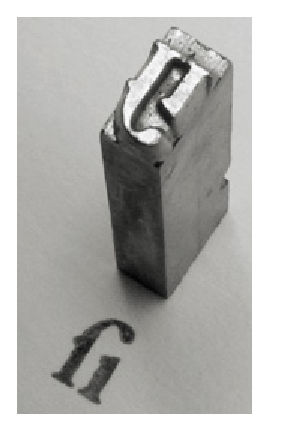
\includegraphics[scale=.5]{resources/ligature}}
        \end{figure}
}
\end{slide}

\begin{slide}{\Large A situação atual}
  % \twocolumn{
  \onslide{1-}{Quais são os problemas encontrados no que diz respeito a:}
  \vspace{1.5cm}
  
  \onslide{2-}{Velocidade}
  \vspace{1cm}
  
  \onslide{3-}{Segurança/Falhas}
  \vspace{1cm}
  
  \onslide{4-}{Controle}
  \vspace{1cm}
  
  \onslide{5-}{TEMPO}
\end{slide}

\begin{slide}{\Large A solução}
   \vspace{.2cm}
\twocolumn{
{   \onslide{2-}{\Large Donald Knuth}
   \vspace{1.5cm}}
   
   \onslide*{4-}{The Art of Computer Programming}
   \vspace{1.5cm}

   {\onslide*{5-}{\LARGE\TeX}}
   
   \begin{figure}[!h]
     \onslide*{3}{
\includegraphics[scale=.14]{resources/taocp}}
   \end{figure}
   \vspace{1.5cm}
}
{
        \begin{figure}[!h]
          \onslide*{2}{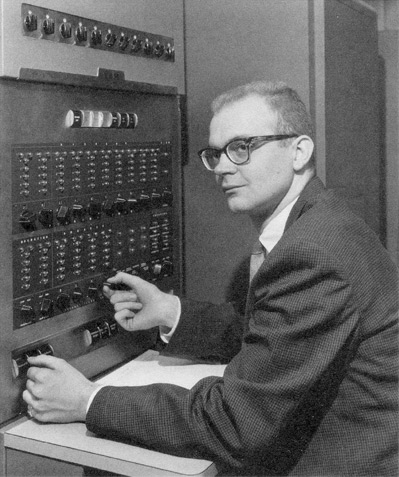
\includegraphics[scale=.3]{resources/youngknuth}}
          \onslide*{3}{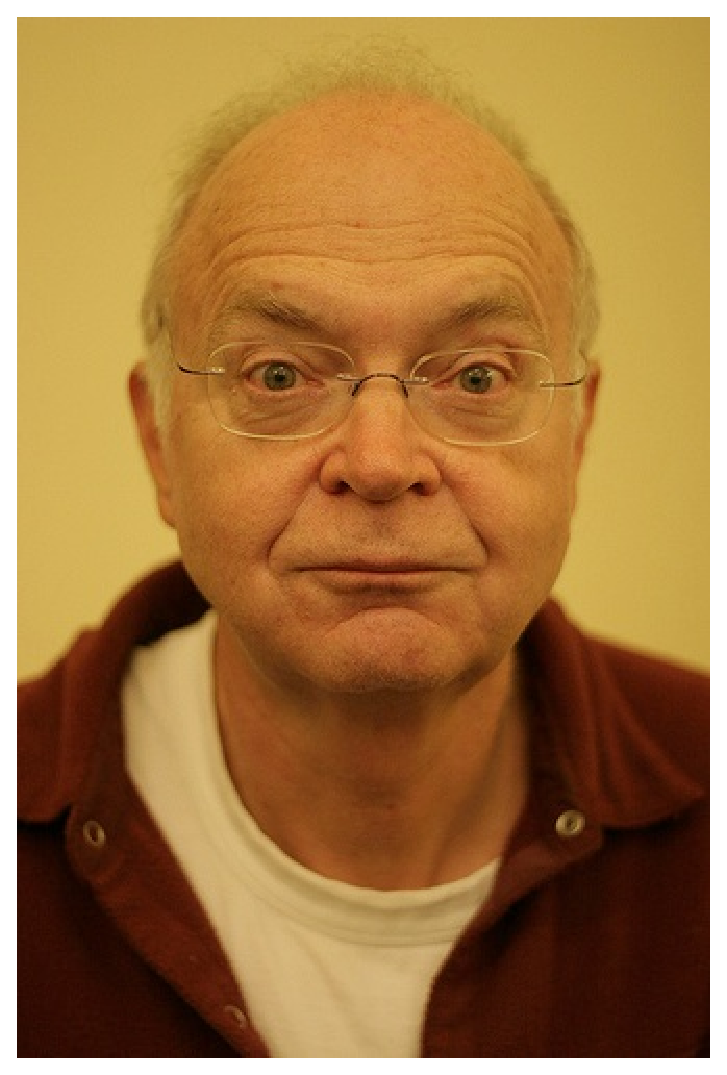
\includegraphics[scale=.3]{resources/knuth}}
        \end{figure}
}

\end{slide}

\end{document}